\section{Results}
\label{sec:results}

\subsection{Baselines: Sequential Training Loses Most of What It Gains}
\label{sec:baselines}

\begin{table}[t]
    \centering
    \small
    \resizebox{\textwidth}{!}{%
    \begin{tabular}{@{}lcccc@{}}
        \toprule
        & \textbf{Zero-shot} & \textbf{End of own stage} & \textbf{Sequential, end of run} & \textbf{Joint multi-task} \\
        \midrule
        \multicolumn{5}{@{}l}{\textit{Mean over six tasks}} \\
        \llama (12 runs; joint 2 seeds) & 0.460 & {\bf 0.624} & 0.499 & 0.623 \\
        \qwen (6 runs; joint 1 seed) & 0.549 & {\bf 0.644} & 0.567 & 0.622 \\
        \midrule
        \multicolumn{5}{@{}l}{\textit{Per task, \llama}} \\
        \tgsm & {\bf 0.445} & 0.345 & 0.199 {\scriptsize (0.085)} & 0.302 \\
        \tarith & 0.920 & 0.926 & 0.825 {\scriptsize (0.165)} & {\bf 0.942} \\
        \tlogic & 0.490 & 0.682 & 0.523 {\scriptsize (0.179)} & {\bf 0.765} \\
        \tmt & 0.403 & {\bf 0.491} & 0.354 {\scriptsize (0.148)} & 0.481 \\
        \tsumm & 0.246 & {\bf 0.404} & 0.271 {\scriptsize (0.112)} & 0.395 \\
        \temo & 0.255 & {\bf 0.896} & 0.820 {\scriptsize (0.049)} & 0.852 \\
        \bottomrule
    \end{tabular}
    }
    \caption{Task metrics for the baselines and for sequential training at the end of the run (standard deviation over runs in parentheses). Best value per row in {\bf bold}. Joint training matches the end-of-own-stage level on average, and sequential training ends close to the zero-shot average. Fine-tuning lowers \tgsm accuracy below zero-shot.}
    \label{tab:baselines}
\end{table}


\Tabref{tab:baselines} compares sequential training with the baselines.
Joint training matches the end-of-own-stage level (0.623 vs.\ 0.624 on \llama; 0.622 vs.\ 0.644 on \qwen), so the sequential shortfall is forgetting and not a capacity limit of the adapter.
Sequential training ends close to the zero-shot average (0.499 vs.\ 0.460 on \llama; 0.567 vs.\ 0.549 on \qwen): most of what fine-tuning added is gone by the end of the run.
Mean backward transfer is $-0.150$ metric units on \llama and $-0.093$ on \qwen.

One baseline result shapes the rest of the analysis.
Fine-tuning \emph{lowers} \tgsm accuracy below zero-shot on \llama (0.445 $\rightarrow$ 0.345).
The raw outputs show why: the zero-shot model writes a long step-by-step solution (mean 657 characters), while the fine-tuned model imitates the terse GSM8K reference style (mean 231 characters) and makes more arithmetic slips.
This is a property of the training targets, not a scoring bug.
It means that \rgain is undefined for \tgsm and \tarith, which show no positive gain, and on \qwen also for \tmt (per-task \qwen values are in \tabref{tab:qwen_baselines}).

\subsection{H1: Forgetting Is a Fast Step at Each Switch, Not a Power Law}
\label{sec:h1}

\begin{figure}[t]
    \centering
    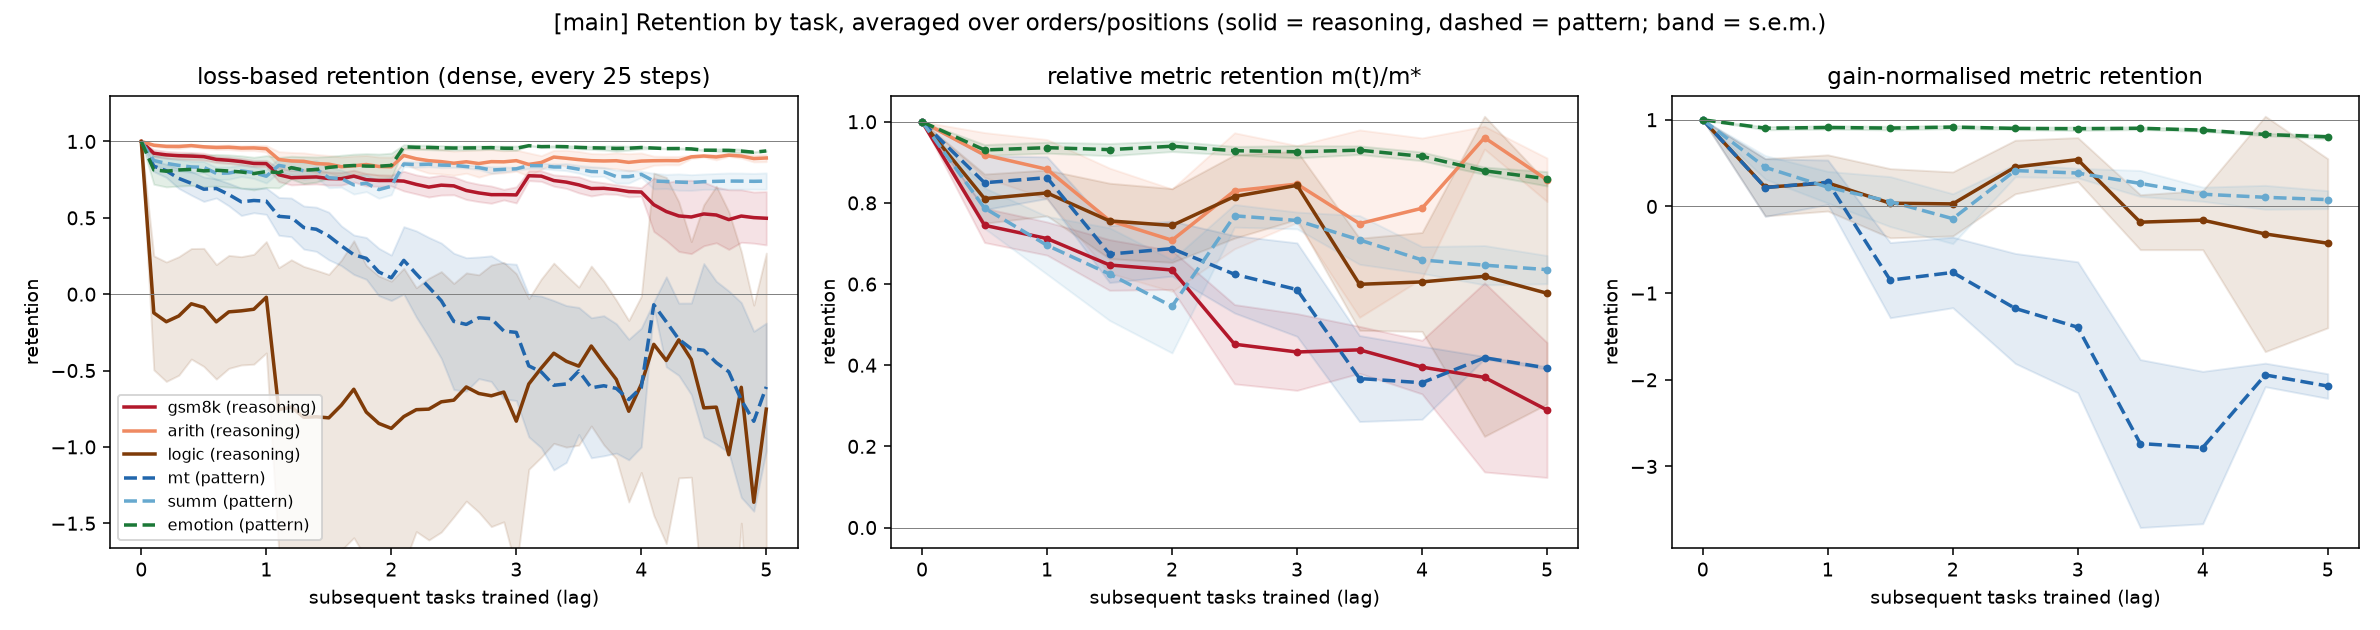
\includegraphics[width=\linewidth]{figures/main_retention_by_task.png}
    \caption{Retention by task on \llama, averaged over orders and positions (solid: reasoning; dashed: pattern; bands: s.e.m.). \figleft~Loss-based retention, every 25 steps. \figcenter~Relative metric retention. \figright~Gain-normalized retention (\tlogic, \tmt, \tsumm, \temo only). Several curves drop sharply right after a stage boundary (integer lags) and are flat, or even rising, for long stretches in between. \tlogic falls below zero-shot level in loss terms soon after the first switch.}
    \label{fig:retention}
\end{figure}

\begin{figure}[t]
    \centering
    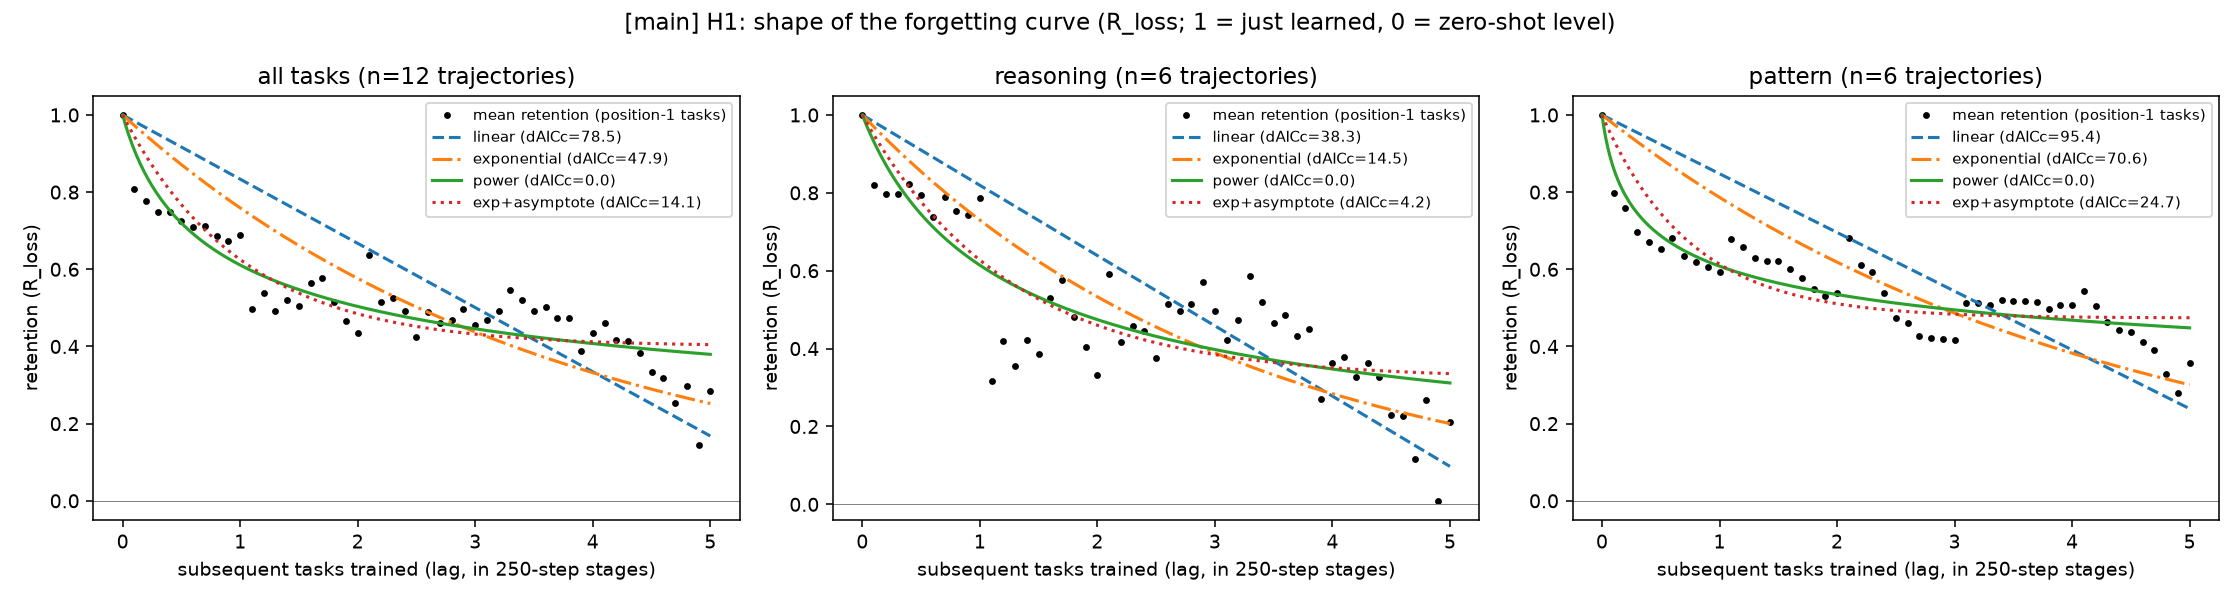
\includegraphics[width=\linewidth]{figures/main_h1_shape_R_loss.png}
    \caption{H1 fits to mean \rloss curves of position-1 tasks on \llama. The power law has the lowest AICc in all three panels, but the data points show steps at stage boundaries that no smooth monotone curve captures.}
    \label{fig:h1}
\end{figure}

\begin{table}[t]
    \centering
    \small
    \resizebox{\textwidth}{!}{%
    \begin{tabular}{@{}lccccc@{}}
        \toprule
        \textbf{Mean curve} & \textbf{Linear} & \textbf{Exponential} & \textbf{Power} & \textbf{Exp+asymptote} & \textbf{$R^2$ of best} \\
        \midrule
        \llama, all tasks, \rloss (12 traj.) & 78.5 & 47.9 & {\bf 0} & 14.1 & 0.81 \\
        \llama, reasoning, \rloss & 38.3 & 14.5 & {\bf 0} & 4.2 & 0.68 \\
        \llama, pattern, \rloss & 95.4 & 70.6 & {\bf 0} & 24.7 & 0.78 \\
        \llama, all tasks, \rrel (11 points) & 27.1 & 23.6 & {\bf 0} & 5.0 & 0.94 \\
        \midrule
        \qwen, all tasks, \rloss (6 traj.) & 82.5 & 28.9 & 8.7 & {\bf 0} & 0.35 \\
        \qwen, reasoning, \rloss & 54.7 & 46.8 & 6.6 & {\bf 0} & 0.08 \\
        \qwen, pattern, \rloss & 61.7 & {\bf 0} & 2.6 & 1.1 & 0.49 \\
        \bottomrule
    \end{tabular}
    }
    \caption{H1 on mean curves of position-1 tasks (pre-registered; lag axis in stages; 51 points per \rloss curve). Entries are \daicc relative to the best model ({\bf 0}); lower is better. The power law wins on the \llama averages and loses on the \qwen averages, where no smooth curve fits well.}
    \label{tab:h1_mean}
\end{table}

\begin{table}[t]
    \centering
    \small
    \begin{tabular}{@{}lcccc@{}}
        \toprule
        \textbf{Trajectories (positions 1--3)} & \textbf{Linear} & \textbf{Exponential} & \textbf{Power} & \textbf{Exp+asymptote} \\
        \midrule
        \llama, \rloss (36) & 9 & 4 & 2 & {\bf 21} \\
        \llama, \rrel (36) & 9 & {\bf 16} & 3 & 8 \\
        \qwen, \rloss (18) & 2 & 4 & 2 & {\bf 10} \\
        \qwen, \rrel (18) & 5 & {\bf 6} & 3 & 4 \\
        \bottomrule
    \end{tabular}
    \caption{H1 on individual trajectories: number of trajectories for which each model has the lowest AICc. Most frequent winner in {\bf bold}. The power law is the least frequent winner, or tied for it, in every row.}
    \label{tab:h1_traj}
\end{table}


{\bf Does the mean curve follow a power law?}
On \llama, yes; on \qwen, no.
\Tabref{tab:h1_mean} shows that linear decay is the worst model in every row, so uniform degradation is clearly rejected.
The power law wins all four \llama mean curves, with a margin of 4.2 to 24.7 AICc units over the saturating exponential.
On \qwen it wins none, and none of the four smooth curves fits well ($R^2 \leq 0.49$).
\Figref{fig:h1} shows the \llama fits.

{\bf Do individual trajectories follow a power law?}
No.
\Tabref{tab:h1_traj} shows that the power law has the lowest AICc in only 2 of 36 \llama trajectories and 2 of 18 \qwen trajectories under \rloss.
The power law and the exponential-to-asymptote both have two parameters, so we also compare just these two (exploratory).
On \llama the saturating exponential is clearly better ($\daicc > 2$) in 26 of 36 trajectories, the power law in 0, with 10 undecided; on \qwen the counts are 9, 2, and 7.
The per-task mean curves agree: the exponential-to-asymptote is best for 5 of 6 tasks on each model.
The power law therefore describes the average better than it describes the things being averaged.

{\bf Why do smooth curves fit poorly?}
Because forgetting comes in steps (\figref{fig:retention}).
We take all stage transitions in which an old task's loss rose by more than 0.02 nats over the stage (108 on \llama, 47 on \qwen).
On \llama the median share of the stage's rise that had already happened at the first evaluation, 25 of 250 steps in, is 55\%, and 72\% by step 50.
Uniform degradation predicts 10\% and 20\%.
On \qwen the shares are 39\% and 66\%.
The curves are also not monotone: in 21\% (\llama) and 24\% (\qwen) of all stage transitions an old task's loss went \emph{down} by more than 0.01 nats.
\Figref{fig:within} shows the mean loss increase within the first interfering stage.
On this within-stage mean the best fit is a power law with a very small exponent (0.07), which is itself close to a step; per trajectory, the saturating exponential wins most often (26 of 54, against 18 for the power law).
At 25-step resolution the two forms are hard to tell apart, which motivated the onset experiment.

\begin{figure}[t]
    \centering
    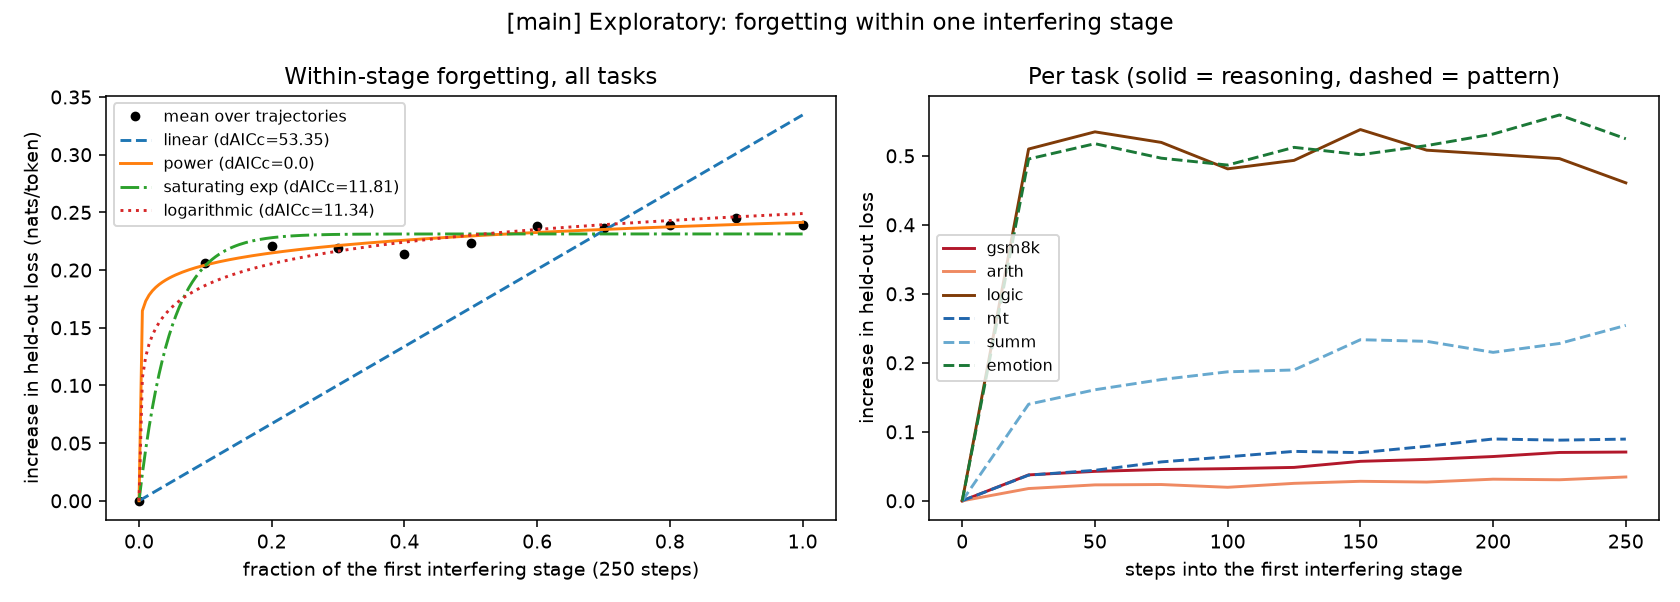
\includegraphics[width=0.95\linewidth]{figures/main_within_stage.png}
    \caption{Forgetting within the first interfering stage on \llama (exploratory). \figleft~Mean increase in old-task loss with four fits; almost all of the increase is present at the first evaluation point. \figright~The same by task. The step is large for \tlogic and \temo and small for \tgsm, \tarith, and \tmt.}
    \label{fig:within}
\end{figure}

\begin{figure}[t]
    \centering
    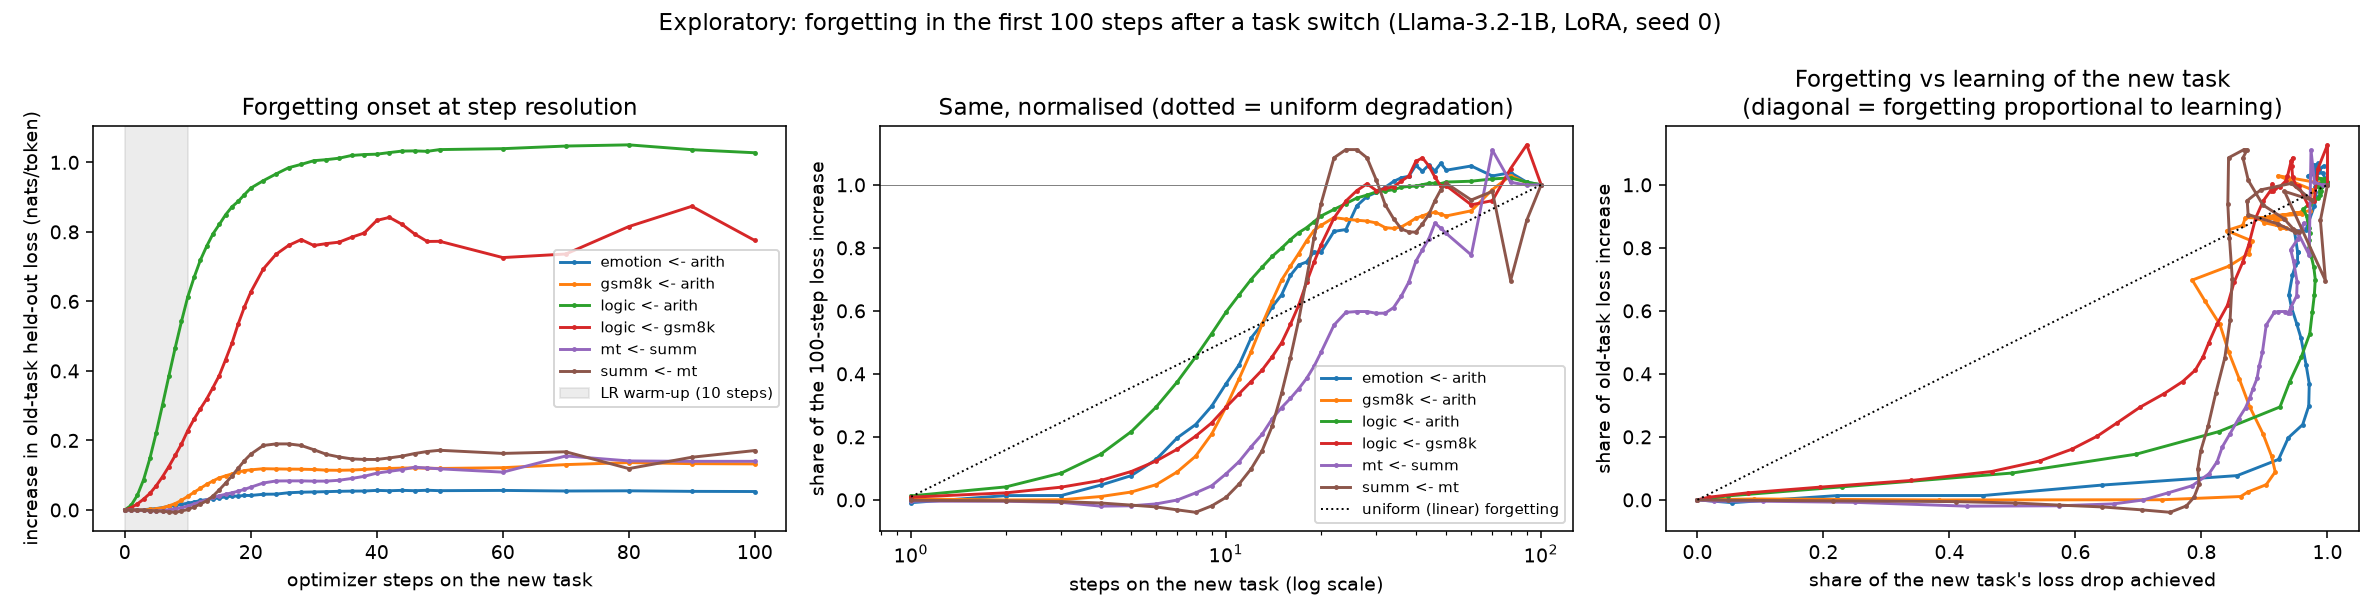
\includegraphics[width=\linewidth]{figures/onset.png}
    \caption{Onset of forgetting at step resolution (exploratory; \llama, six pairs, one seed). \figleft~Increase in old-task loss during the first 100 steps on a new task; the shaded region is the 10-step learning-rate warm-up. \figcenter~The same, normalized by the 100-step increase, on a log axis; the dotted line is uniform degradation. \figright~Forgetting of the old task against learning of the new task; forgetting lags behind learning.}
    \label{fig:onset}
\end{figure}

\begin{table}[t]
    \centering
    \resizebox{\textwidth}{!}{%
    \begin{tabular}{@{}lccccc@{}}
        \toprule
        & \textbf{Loss rise after} & \textbf{Share of rise reached} & \textbf{Old task: steps to} & \textbf{New task: steps to} & \textbf{\daicc, power vs.} \\
        \textbf{Old $\leftarrow$ new} & \textbf{100 steps (nats/token)} & \textbf{by step 10 / 20 / 50} & \textbf{50\% / 90\% of rise} & \textbf{50\% / 90\% of drop} & \textbf{saturating exp.} \\
        \midrule
        \tlogic $\leftarrow$ \tarith & 1.028 & 0.60 / 0.90 / 1.01 & 9 / 20 & 4 / 6 & $+74.9$ \\
        \tlogic $\leftarrow$ \tgsm & 0.775 & 0.29 / 0.81 / 1.00 & 16 / 24 & 6 / 26 & $+38.4$ \\
        \tsumm $\leftarrow$ \tmt & 0.171 & 0.01 / 0.94 / 1.00 & 17 / 20 & 4 / 34 & $+15.0$ \\
        \tmt $\leftarrow$ \tsumm & 0.140 & 0.08 / 0.47 / 0.85 & 22 / 70 & 5 / 22 & $+21.0$ \\
        \tgsm $\leftarrow$ \tarith & 0.132 & 0.30 / 0.87 / 0.90 & 13 / 42 & 3 / 6 & $+31.5$ \\
        \temo $\leftarrow$ \tarith & 0.053 & 0.37 / 0.79 / 1.05 & 12 / 26 & 4 / 6 & $+52.0$ \\
        \bottomrule
    \end{tabular}
    }
    \caption{Step-resolution onset of forgetting (exploratory; \llama, one seed). Positive \daicc means the saturating exponential fits better than the power law. Forgetting is mostly complete by step 20--50 and lags behind learning of the new task.}
    \label{tab:onset}
\end{table}


{\bf What does the onset look like at step resolution?}
\Figref{fig:onset} and \tabref{tab:onset} show the six pairs.
The saturating exponential is the best of the four candidates in all six pairs, and linear is the worst in all six (\daicc 32--149).
Between step 50 and step 100 the old-task loss changes by at most 0.022 nats.
The curves are slightly S-shaped: almost nothing happens in the first $\sim$5 steps, which coincides with the 10-step warm-up.
Forgetting also lags behind learning: the new task reaches half of its loss drop in 3--6 steps, the old task half of its loss rise in 9--22.
The warm-up is a property of our training recipe, so the delay may not generalize.

\para{Verdict on H1: not supported as stated.}
``Not uniform'' holds strongly.
``Power law'' holds only for averaged curves on one of two models.
The data are better described as a rapid, saturating step at each task switch whose size varies by task pair.
Summing such steps over a balanced set of interferers would give a decelerating average curve that a power law fits well; this reading is consistent with the fits above, but we did not test it directly.

\subsection{H2: No 3--5$\times$ Gap Between Reasoning and Pattern Tasks}
\label{sec:h2}

\begin{table}[t]
    \centering
    \resizebox{\textwidth}{!}{%
    \begin{tabular}{@{}lcccc@{}}
        \toprule
        & \multicolumn{2}{c}{\llama (12 runs)} & \multicolumn{2}{c}{\qwen (6 runs)} \\
        \cmidrule(lr){2-3} \cmidrule(lr){4-5}
        \textbf{Measure} & \textbf{Reas.\ / patt.} & \textbf{Ratio [95\% CI]} & \textbf{Reas.\ / patt.} & \textbf{Ratio [95\% CI]} \\
        \midrule
        \rloss (pre-registered) & 0.637 / 0.434 & 1.47 [1.05, 1.91] & 0.610 / 0.103 & 5.93 [$-12.9$, 32.5] \\
        \rrel (pre-registered) & 0.286 / 0.251 & 1.14 [0.82, 1.60] & 0.210 / 0.096 & 2.18 [1.08, 3.52] \\
        \rgain (pre-registered)$^\dagger$ & 0.843 / 0.954 & 0.88 [0.39, 1.56] & 0.505 / 0.399 & 1.27 [$-0.05$, 3.25] \\
        \absdrop & 0.165 / 0.124 & 1.33 [0.89, 1.90] & 0.157 / 0.060 & 2.60 [1.21, 4.21] \\
        \rloss clipped to $[0,1]$ (exploratory) & 0.349 / 0.347 & 1.01 [0.82, 1.26] & 0.453 / 0.374 & 1.21 [0.72, 1.95] \\
        \bottomrule
    \end{tabular}
    }
    \caption{H2: mean forgetting for reasoning and pattern tasks and their ratio, with cluster-bootstrap 95\% intervals over runs. Forgetting is $1 - R$ (or the absolute drop), averaged over all stage-end evaluations with lag $\geq 1$. H2 predicts a ratio in $[3, 5]$. $^\dagger$\tgsm and \tarith are excluded on both models and \tmt on \qwen, because fine-tuning gave no positive gain.}
    \label{tab:h2_ratio}
\end{table}

\begin{table}[t]
    \centering
    \small
    \begin{tabular}{@{}llcccccc@{}}
        \toprule
        & & \multicolumn{3}{c}{\llama} & \multicolumn{3}{c}{\qwen} \\
        \cmidrule(lr){3-5} \cmidrule(lr){6-8}
        \textbf{Task} & \textbf{Cat.} & \absdrop & $1-\rrel$ & $1-\rloss$ & \absdrop & $1-\rrel$ & $1-\rloss$ \\
        \midrule
        \tgsm & R & 0.153 & {\bf 0.435} & 0.264 & 0.104 & 0.231 & {\bf 0.954} \\
        \tarith & R & 0.168 & 0.186 & 0.109 & {\bf 0.282} & {\bf 0.288} & 0.562 \\
        \tlogic & R & {\bf 0.173} & 0.239 & {\bf 1.536} & 0.084 & 0.111 & 0.313 \\
        \tmt & P & 0.167 & 0.338 & 0.940 & 0.027 & 0.057 & $-0.044$ \\
        \tsumm & P & 0.139 & 0.341 & 0.236 & 0.034 & 0.100 & 0.215 \\
        \temo & P & 0.066 & 0.073 & 0.126 & 0.120 & 0.131 & 0.138 \\
        \bottomrule
    \end{tabular}
    \caption{Per-task forgetting (R = reasoning, P = pattern). Largest forgetting per column in {\bf bold}. Differences between tasks within a category are larger than the difference between categories, and the two models disagree on which tasks are fragile.}
    \label{tab:h2_pertask}
\end{table}


\Tabref{tab:h2_ratio} gives the category ratio under five measures, and \tabref{tab:h2_pertask} gives the per-task values behind it.

\para{\llama.}
No measure comes near 3.
The only interval that excludes 1 is unclipped \rloss (ratio 1.47; bootstrap one-sided $p = 0.016$, Holm-adjusted $p = 0.049$ over the three pre-registered measures).
One task carries this result: \tlogic spends 43\% of its cells \emph{below zero-shot level} in loss terms, and without \tlogic the ratio is 0.43.
Clipping gives 1.01.
The task-label permutation test gives $p = 0.7$.
In metric terms the three reasoning tasks and two of the three pattern tasks lose about the same (0.14--0.17); only \temo is robust.

\para{\qwen.}
The metric-based ratios are above 2, and their intervals exclude 1 (one-sided $p = 0.019$ for \rrel and $0.017$ for \absdrop) and overlap $[3, 5]$.
After Holm correction the \rrel result is $p = 0.057$.
The task-label permutation test gives $p = 0.2$--$0.3$; the smallest attainable value with six tasks is 0.1.
The unclipped loss ratio of 5.93 is not interpretable: \qwen barely improves on \tmt and \tgsm in loss terms ($L_0 - L^* = 0.033$ and $0.078$ nats), so the normalization divides by nearly zero, as the interval $[-12.9, 32.5]$ shows.
The largest metric drop on \qwen is \tarith (0.282) and the smallest are \tmt and \tsumm (about 0.03), but \qwen also gained almost nothing on \tmt from fine-tuning, so there was little to lose.

\para{Verdict on H2: not supported.}
A 3--5$\times$ gap is absent on \llama under every normalization.
\qwen shows a roughly 2.2--2.6$\times$ gap on metric-based measures that is suggestive but not robust to correction, to the choice of normalization, or to treating tasks instead of runs as the unit of generalization.
With three tasks per category, we cannot separate ``reasoning vs.\ pattern'' from ``these particular tasks''.

\subsection{H3: No Reliable Effect of Serial Position}
\label{sec:h3}

\begin{figure}[t]
    \centering
    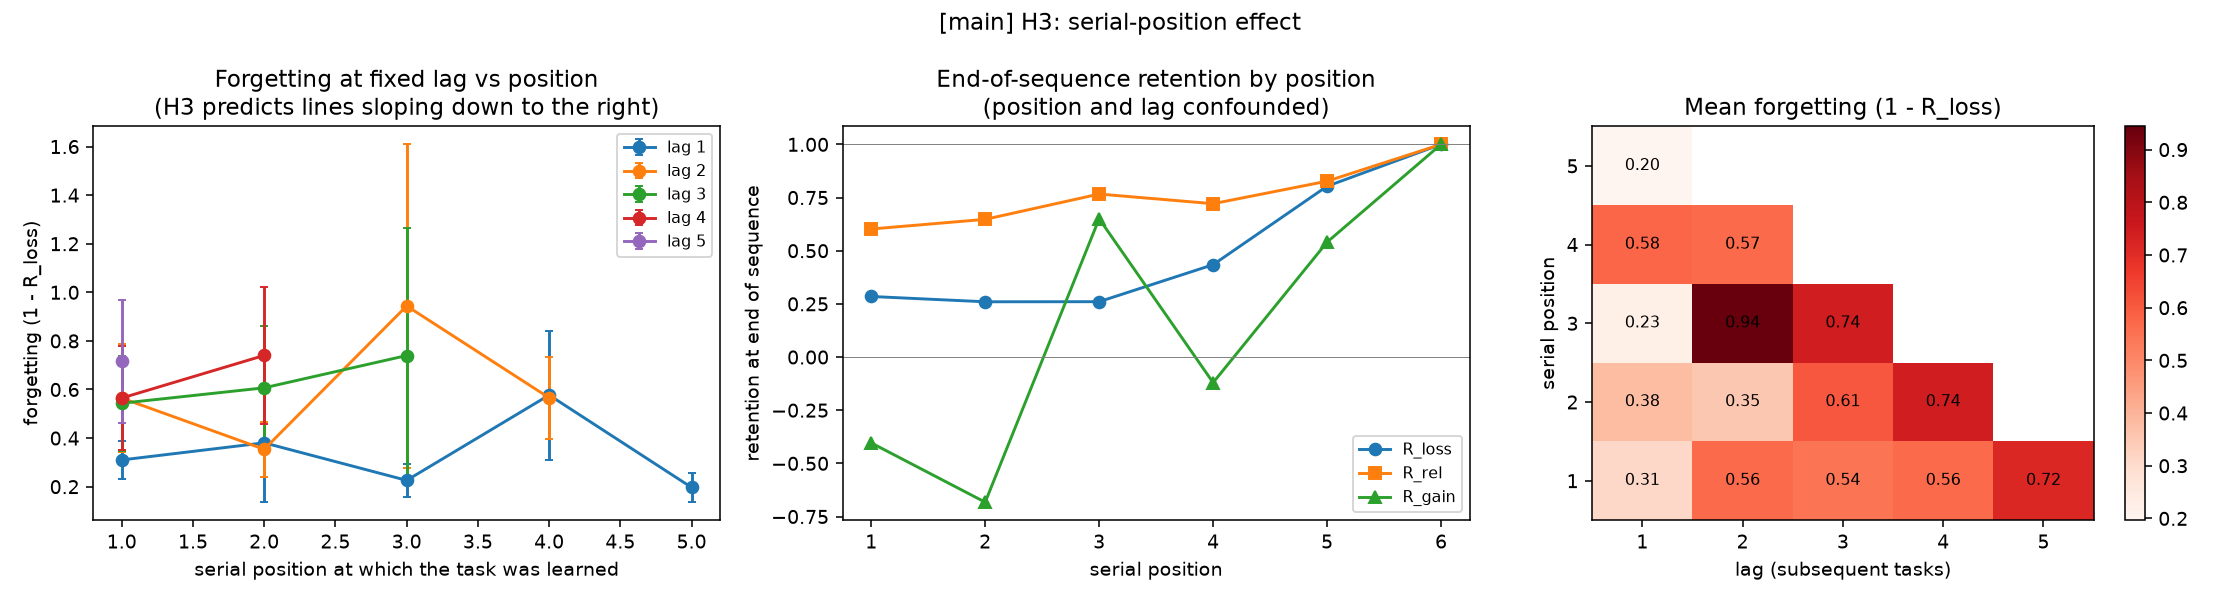
\includegraphics[width=\linewidth]{figures/main_h3_position.png}
    \caption{H3 on \llama, using unclipped \rloss. \figleft~Forgetting at fixed lag against serial position; H3 predicts lines sloping down to the right, which we do not see. \figcenter~End-of-sequence retention rises with position, but position and lag are confounded there. \figright~Mean forgetting by position and lag.}
    \label{fig:h3}
\end{figure}

\begin{table}[t]
    \centering
    \resizebox{\textwidth}{!}{%
    \begin{tabular}{@{}lcc@{}}
        \toprule
        & \llama (12 runs) & \qwen (6 runs) \\
        \midrule
        Lag-1 forgetting by position 1--5, \rloss clipped & 0.31, 0.21, 0.23, 0.38, 0.20 & 0.55, 0.51, 0.29, 0.23, 0.15 \\
        Spearman, position vs.\ lag-1 forgetting, \rloss clipped & $\rho = -0.06$, $p = 0.65$ & $\rho = -0.47$, $p = 0.009$ \\
        Same, \rrel & $\rho = 0.02$, $p = 0.87$ & $\rho = -0.18$, $p = 0.34$ \\
        Same, \rloss unclipped & $\rho = -0.12$, $p = 0.37$ & $\rho = -0.35$, $p = 0.055$ \\
        \midrule
        OLS position coefficient, \rloss clipped [95\% CI] & $-0.001$ [$-0.028$, 0.026] & $-0.073$ [$-0.138$, $-0.009$] \\
        OLS position coefficient, \rrel [95\% CI] & $-0.019$ [$-0.063$, 0.025] & $-0.019$ [$-0.047$, 0.009] \\
        OLS $\log(1+\text{lag})$ coefficient, \rrel [95\% CI] & 0.154 [0.015, 0.294] & $-0.039$ [$-0.206$, 0.128] \\
        \bottomrule
    \end{tabular}
    }
    \caption{H3: effect of serial position with lag held fixed. Spearman correlations use task-demeaned forgetting. A negative position coefficient is the direction H3 predicts (earlier-learned tasks forget more at the same lag). The $p$-values are uncorrected.}
    \label{tab:h3}
\end{table}


End-of-sequence retention does rise with position on both models; on \llama, \rrel is 0.60, 0.65, 0.77, 0.72, and 0.83 for positions 1--5 (\figref{fig:h3}, center).
But there, position and amount of subsequent training are the same thing.
\Tabref{tab:h3} holds lag fixed.

\llama shows no position effect on any measure: the Spearman correlations are between $-0.12$ and $0.02$, and both OLS position coefficients have intervals centered near zero.
\qwen shows the predicted direction on the clipped loss measure ($\rho = -0.47$, $p = 0.009$; OLS coefficient $-0.073$) and the same sign without significance on the metric measure.
These $p$-values are uncorrected across measures and models, and cluster-robust errors with six clusters are unreliable.

The two models also differ in how forgetting accumulates.
On \llama forgetting keeps growing with lag (log-lag coefficient 0.154 for \rrel).
On \qwen it does not measurably grow after the first subsequent task (coefficient $-0.039$, interval spanning zero).

\para{Verdict on H3: not supported on \llama; inconclusive on \qwen.}
On \llama the visible end-of-run disadvantage of early tasks is explained by their longer exposure to interference.

\subsection{What Does Predict Forgetting? Pair Structure and Output Format}
\label{sec:pairs}

\begin{table}[t]
    \centering
    \small
    \begin{tabular}{@{}lcccccc@{}}
        \toprule
        \textbf{Old $\backslash$ new} & \tgsm & \tarith & \tlogic & \tmt & \tsumm & \temo \\
        \midrule
        \tgsm & -- & 0.21 & 0.17 & 0.03 & 0.04 & 0.05 \\
        \tarith & 0.00 & -- & 0.16 & $-0.05$ & $-0.09$ & 0.14 \\
        \tlogic & {\bf 1.11} & {\bf 1.63} & -- & $-0.57$ & {\bf 0.91} & $-0.18$ \\
        \tmt & $-0.01$ & $-0.04$ & 0.14 & -- & {\bf 0.78} & {\bf 0.83} \\
        \tsumm & $-0.03$ & 0.02 & 0.13 & 0.17 & -- & 0.12 \\
        \temo & $-0.02$ & 0.19 & 0.04 & 0.02 & 0.02 & -- \\
        \bottomrule
    \end{tabular}
    \caption{Pair structure on \llama: mean loss-based retention (\rloss) lost by an old task (row) during one stage of training on a new task (column). Negative values are recovery. The five largest cells are in {\bf bold}; they carry most of the forgetting.}
    \label{tab:interference}
\end{table}

\begin{table}[t]
    \centering
    \small
    \begin{tabular}{@{}lccc@{}}
        \toprule
        & \multicolumn{2}{c}{\llama} & \qwen \\
        \cmidrule(lr){2-3} \cmidrule(lr){4-4}
        \textbf{Task} & \textbf{Format valid} & \textbf{Score given valid format} & \textbf{Format valid} \\
        \midrule
        \tgsm & 0.99 $\rightarrow$ 0.70 & 0.35 $\rightarrow$ 0.21 & 1.00 $\rightarrow$ 0.75 \\
        \tarith & 1.00 $\rightarrow$ 0.73 & 0.93 $\rightarrow$ 0.79 & 1.00 $\rightarrow$ 0.68 \\
        \tlogic & 1.00 $\rightarrow$ 0.73 & 0.68 $\rightarrow$ 0.61 & 1.00 $\rightarrow$ 0.96 \\
        \tmt & 0.99 $\rightarrow$ 0.62 & 0.49 $\rightarrow$ 0.36 & 1.00 $\rightarrow$ 0.99 \\
        \tsumm & 1.00 $\rightarrow$ 0.75 & 0.40 $\rightarrow$ 0.28 & 1.00 $\rightarrow$ 0.96 \\
        \temo & 1.00 $\rightarrow$ 0.87 & 0.90 $\rightarrow$ 0.84 & 1.00 $\rightarrow$ 0.99 \\
        \bottomrule
    \end{tabular}
    \caption{Format versus content. Each entry is (just learned $\rightarrow$ after later tasks). ``Format valid'' is the share of outputs with the requested form (\eg contains \texttt{Answer:}, is one of the allowed labels, is not an echo of the source). On \llama both the output format and the score among well-formatted outputs erode.}
    \label{tab:format}
\end{table}


\para{Pair structure.}
\Tabref{tab:interference} shows how much retention each old task loses during one stage of each new task on \llama.
A handful of pairs carry most of the forgetting: \tlogic after \tarith, \tgsm, or \tsumm, and \tmt after \tsumm or \temo.
Some pairs produce recovery, such as \tlogic after \tmt ($-0.57$).
On \llama, same-category pairs average 0.435 against 0.039 for cross-category pairs.
This contrast rests on those few cells and does not replicate on \qwen ($-0.219$ vs.\ 0.023), where the \tmt row is distorted by the near-zero loss denominator.
On \qwen, \tlogic is the most damaging \emph{interferer} and not the most damaged task (\tabref{tab:qwen_interference}).

\para{Format versus content.}
We check each stored generation for the requested output form (\tabref{tab:format}).
On \llama every task loses its output format in 13--38\% of later outputs, and the score also falls among outputs that keep the format.
Both the interface and the content erode.
On \qwen, format loss is confined to \tgsm and \tarith, the two tasks with multi-line worked answers.
Typical failures after a later task has been trained are an arithmetic answer written as prose without the \texttt{Answer:} line after summarization training, and a GSM8K problem that is paraphrased instead of solved.
